\documentclass{article}

\usepackage{graphicx}
\usepackage{hyperref}
\usepackage{siunitx}
\usepackage{todonotes}

\title{Electronics Lab}

\begin{document}

\listoftodos
\newpage

\maketitle

\todo{Introduction}
\todo{Men}

\section{Setup}

On your desk you should find:

\begin{itemize}
\item a breadboard (a white plastic board with a grid of holes)
\item pliers
\item wire strippers
\item wire cutters
\item a PP3 (9 volt) battery
\item a clip for the battery
\item two LEDs (one red, one green)
\item two resistors
\item a microswitch
\end{itemize}

\todo[inline]{Describe these components in more detail, or add images}
\todo[inline]{Ensure this is up to date}

If some of these items aren't present or if you're having trouble identifying
them, please ask for assistance from one of the mentors.

\subsection{Hookup wire}

We will use single-strand hookup wire to connect up our circuit. Some
electronics kits provide pre-cut wires with connectors attached to each end;
however being able to cut and strip wire off the reel is a good skill to learn.

Using the wire cutters, cut roughly \SI{30}{\centi\metre} of black and red wire
from the reels. Conventially, red wire is used for anything directly connected
to the positive power supply and black wire is used for anything directly
connected to the negative power supply (ground).

Also cut about \SI{60}{\centi\metre} of any other colour. This wire will be used
for any other connections in the circuit. Feel free to use different colours to
represent different sections of the circuit (e.g. blue for input circuitry and
green for output circuitry), or anything else that may help you keep track of
the layout of your circuit better.

Practise cutting a few short lengths of wire and stripping the insulation off
the ends. You should leave between \SI{5}{\milli\metre} and
\SI{10}{\milli\metre} of bare copper at the end; too little and the wire won't
stay securely in the breadboard hole, too much and you risk exposed copper
making contact nearby component leads or other wires and causing a short
circuit. If you are unfamiliar with the process of stripping wires, ask a
mentor to demonstrate the procedure.

\subsection{Breadboard}

In this lab, we will build our circuits on a breadboard, which is a useful
platform for mounting and connecting components that doesn't require soldering.
Some of you may have used a breadboard before; if not, there is an excellent
guide to getting started with breadboards available on SparkFun's website at
\url{https://learn.sparkfun.com/tutorials/how-to-use-a-breadboard}.

The breadboards have two power supply rows at the top, one labelled with
a red line (usually used for the positive power supply) and one with a blue or
black line (for the negative power supply). There are also another two
rows like these at the bottom of the board. Using a piece of (preferably red)
hookup wire, connect the two red rows together. Do the same for the two
black/blue rows with a piece of black wire.

The rest of the holes are the main working area. Each column of five adjacent
holes is electrically connected together.

\subsection{Battery clip}

For this lab we'll use a standard PP3 (9 volt) battery as our power supply.
Grab the battery clip and strip the ends of the leads if necessary. Plug the
red (positive) lead into one of the positive power supply rows of the
breadboard, and the black (negative) lead into one of the negative power supply
rows.

Don't connect the clip to the battery just yet; we'll do that when we're ready
to test our circuit. It's good practice to keep the power to your circuit
disconnected except when necessary.

\section{Lighting an LED}

Let's set up a simple circuit to light up an LED. There are a couple of things
to consider when using LEDs in circuits. The first is their \emph{polarity},
which refers to which way round the two leads are connected. One of the leads
is the \emph{anode} and the other is the \emph{cathode}. To identify which is
which, you can look at either the length of the leads (the cathode is slightly
shorter than the anode) or the lip around the base of the LED body (which is
flat on the cathode's side and curved on the anode's side). The anode should
always be connected to a higher voltage than the cathode in order for the LED
to work.

The other issue is the amount of current flowing through the LED. If it was
connected directly to the power supply, a very large current will flow, which
will almost certainly damage the LED and battery. Therefore, we will add a
\emph{resistor} to the circuit to limit the current. We'll use a
\SI{390}{\ohm} resistor, since that will allow enough current to flow to light
the LED quite brightly.

Place the resistor and red LED in the breadboard so that:

\begin{itemize}
\item one end of the resistor is connected to the positive power supply.
\item the other end of the resistor is connected to the anode of the LED.
\item the cathode of the LED is connected to the negative power supply.
\end{itemize}

Figure~\ref{fig:breadboard:led} shows how this could be done on the breadboard.
The same circuit is shown in Figure~\ref{fig:schem:led} as a schematic diagram.
Schematics are widely used for modelling circuits in a logical manner, without
having to worry about the physical layout of the circuit. The symbols represent
components (the battery, resistor and LED) and the lines between them represent
electrical connections (wires and breadboard connections). Compare the schematic
diagram to the breadboard layout to get a feel for how schematic diagrams work,
since the more complex circuits will be described mainly using their diagrams.

\begin{figure}
\centering
\missingfigure{LED circuit built on a breadboard}
\caption{LED circuit built on a breadboard.}
\label{fig:breadboard:led}
\end{figure}

\begin{figure}
\centering
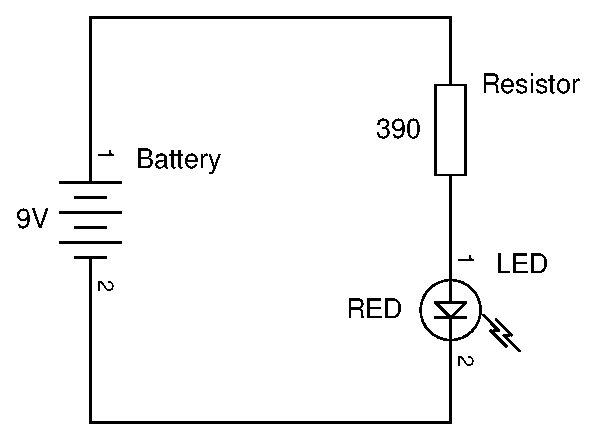
\includegraphics[width=\textwidth]{assets/fig/schem/led}
\caption{Schematic diagram of the LED circuit.}
\label{fig:schem:led}
\end{figure}

Now, when you put the battery clip onto the battery, the LED should light up.
If it does, well done! If it doesn't, have a think about where the problem
could lie.

\begin{itemize}
\item Is the LED connected the right way round?
\item Is the battery clip on the right way round? \todo{How do you know the clip is the right way round?}
\item Are the resistor and LED connected to the same 5-hole group?
\todo{More troubleshooting options would be nice.}
\end{itemize}

If you're still unable to locate the problem, ask a mentor for assistance.

\section{Using a microswitch}

Lighting up an LED is all well and good, but it's not particularly interactive.
Let's add some input to our circuit. We'll use a microswitch (a type of
pushbutton). We'll also add a second LED (a green one), and set up the circuit
so that the green LED lights when the switch is pressed and the red one lights
when it's not pressed.

First, unplug the battery from its clip; it's a good idea to always disconnect
the power from your circuit before you modify it, to reduce the risk of
short-circuiting the battery or damaging the components.

The microswitch has three wires coming out of it: ``common'' (black), ``normally
open'' (blue) and ``normally closed'' (red). When the switch is not being
pressed, ``common'' and ``normally closed'' are connected together inside the
switch, and ``normally open'' is not connected to anything. Likewise when the
switch is pressed, ``common'' and ``normally open'' are connected together and
``normally closed'' is disconnected.

We can use this in our circuit by connecting the LED-and-resistor combinations
to the ``normally open'' and ``normally closed'' terminals of the switch,
instead of directly to the battery. The battery is instead connected to the
``common'' of the switch. When the switch is not pressed, one LED is connected
to the battery via the switch (so it will light up) and the other LED circuit is
disconnected (so it won't light up). Pressing the switch in reverses which LED
is connected and which is disconnected.

The schematic for our circuit is shown in Figure~\ref{fig:schem:switch}. The
switch is the symbol to the above and right of the battery. The connection
labelled with a ``1'' is the ``common'' terminal of the switch (black wire), the
wire labelled ``2'' is the ``normally open'' terminal (blue wire) and the wire
labelled ``3'' is the ``normally closed'' terminal (red wire).

\begin{figure}
\centering
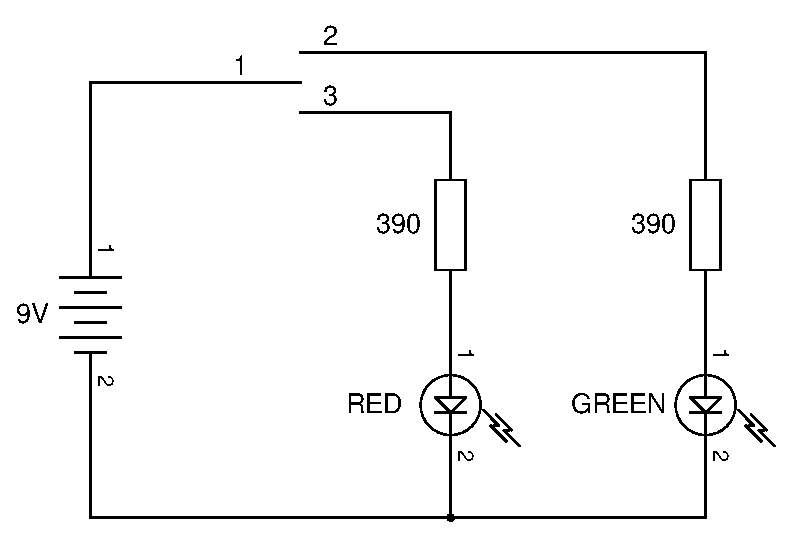
\includegraphics[width=\textwidth]{assets/fig/schem/switch}
\caption{Schematic diagram of the microswitch circuit.}
\label{fig:schem:switch}
\end{figure}

Check that your circuit works before moving on.

\end{document}


% Questions:
%   Are bench PSUs available?
%   Are participants working in pairs or on their own?
%   Should hookup wires be provided, or should participants cut and strip their
%    own wire?
%   Do we need to buy pliers, wire strippers etc. or will ECS loan us these?
